\documentclass{article}
\usepackage[utf8]{inputenc}
\usepackage{graphicx}

\title{Tugas Pemrograman Chapter 4}
\author{Dyah Ayu Anandra (1184098) }
\date{29 Desember 2019}

\begin{document}

\maketitle

\section{Teori}
\subsection{Sejarah dan Contoh Pengelolaan File CSV}
\usepackage{CSV kepanjangan dari Comma Separated Value merupakan salah satu tipe file yang digunakan di dalam dunia programming. Tidak hanya digunakan di dunia programming CSV pun sering digunakan dalam pengolahan informasi yang dihasilkan oleh spreadsheet untuk diproses lebih lanjut melalui mesin analitik. CSV juga dianggap sebagai file yang agnostik karena dapat digunakan oleh berbagai database untuk proses backup data. untuk pengaplikasian dalam bahasa pemrograman python buat terlebih dahulu CSV nya dengan excel kemudian akan dilakukan pemanggilan untuk data yang berada di CSV tersebut. Ada beberapa cara untuk membaca file CSV pada python:}
\begin{center}
    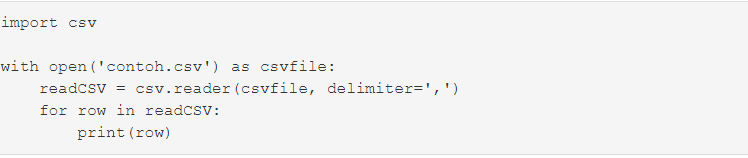
\includegraphics[width = 8cm\textwidth]{cs1.png}
\end{center}

\begin{center}
    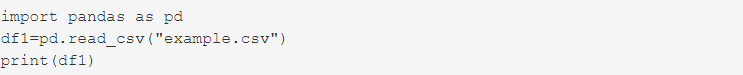
\includegraphics[width = 8cm\textwidth]{cs2.png}
\end{center}

\subsubsection{}
\begin{itemize}
    \item Notepad ++
    \item Microsoft Exel 
    \iteem Google Spreadsheets
    \item  Open Office Calc dan lain-lain.
\end{itemize}

\subsection{Cara Menulis dan Membaca File CSV di Excel atau Spreadsheet}
\begin{enumerate}
    \item Langkah pertama buka lembar baru pada Microsoft Excel
    \item Kemudian ketikkan setiap judul atau nama kolom pada kotak-kotak di baris pertama yang ada di bagian paling atas lembar lajur.
    \item Selanjutnya masukkan data pada lembar lajur di bawah judul di setiap kolom sesuai dengan kebutuhan datanya.
    \item Lalu untuk menyimpan file klik menu “File” dan pilih “Save As” dan memilih folder untuk menyimpan data tersebut.
    \item Tahap selanjutnya pilih “CSV” dari menu drop-down “Save as type” untuk menyimpan file dengan format CSV.
    \item Langkah terakhir ketikkan nama berkas CSV, kemudian pilih “Save”, setelah itu selesai.
\end{enumerate}

\subsection{Libarary CSV}

\begin{center}
    
\includegraphics[width = 8cm\textwidth]{l1.png}
\end{center}

\begin{center}
    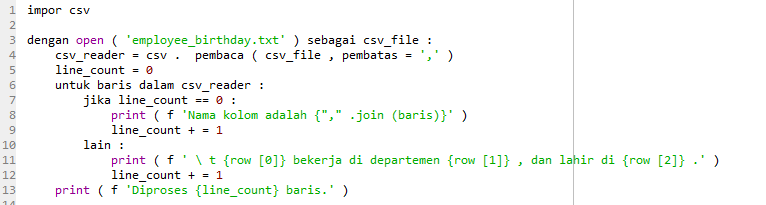
\includegraphics[width = 8cm\textwidth]{l2.png}
\end{center}

\begin{center}
    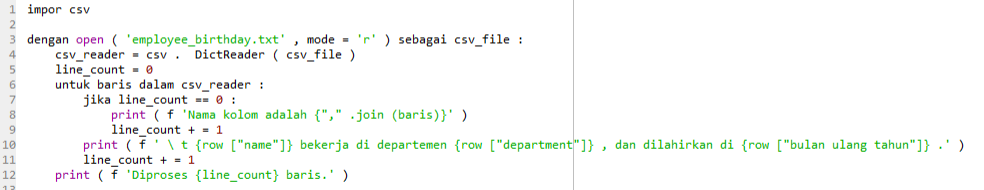
\includegraphics[width = 8cm\textwidth]{l3.png}
\end{center}

\subsection{Library Pandas}

\begin{center}
    
\includegraphics[width = 8cm\textwidth]{p1.png}
\end{center}

\begin{center}
    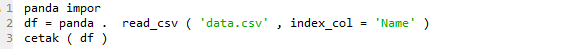
\includegraphics[width = 8cm\textwidth]{p2.png}
\end{center}

\begin{center}
    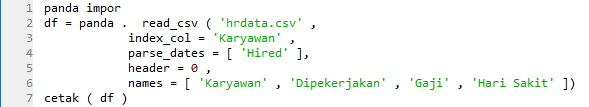
\includegraphics[width = 8cm\textwidth]{p3.png}
\end{center}

\section{Soal}

\begin{center}
    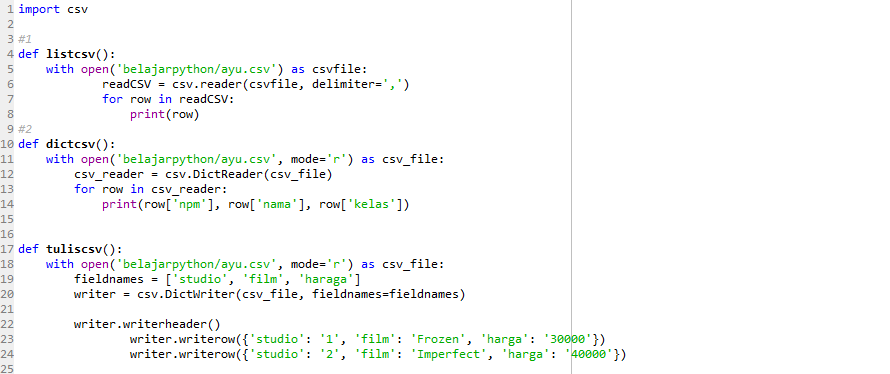
\includegraphics[width = 8cm\textwidth]{so11.png}
\end{center}

\begin{center}
    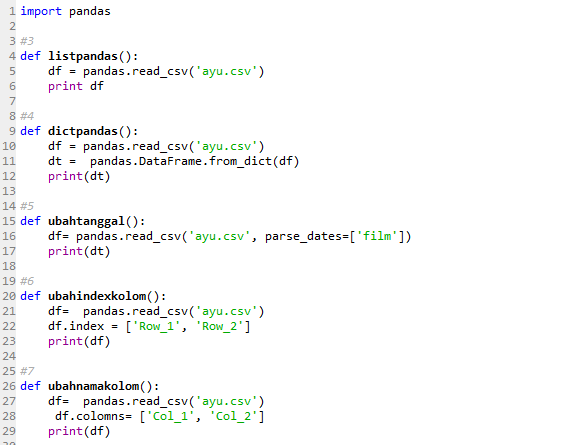
\includegraphics[width = 8cm\textwidth]{so2.png}
\end{center}

\begin{center}
    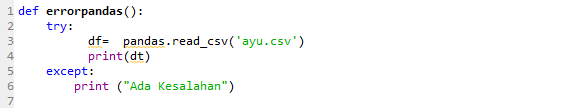
\includegraphics[width = 8cm\textwidth]{so3.png}
\end{center}

\end{document}